\chapter{Grundlagen} \label{chapter_2}
In diesem Kapitel wird zuerst auf das Umfeld der Arbeit im Bereich der Produktkonfiguratoren eingegangen. Das Produkt CAS Merlin Enterprise wird anschließend vorgestellt, sowie auf die kundenspezifischen Konfigurationsprozesse eingegangen. Zum Abschluss werden die Anforderungen der Anwendung dargestellt.

\section{Produktkonfiguratoren}\label{konfiguratoren}
Das Ziel des Produktkonfigurators ist es, produktspezifisches Wissen für die Anwender bereit zu stellen, das ihn bei der individuellen Zusammenstellung des Produktes unterstützt. Ein solches System wird in die Kategorie der Expertensysteme\cite{bib:puppe} oder wissensbasierte Systeme eingeordnet. Der Aufbau eines solches System ist in Abbildung \ref{expert_system_structure} zu sehen. \par
\begin{figure}[hb]
\centering
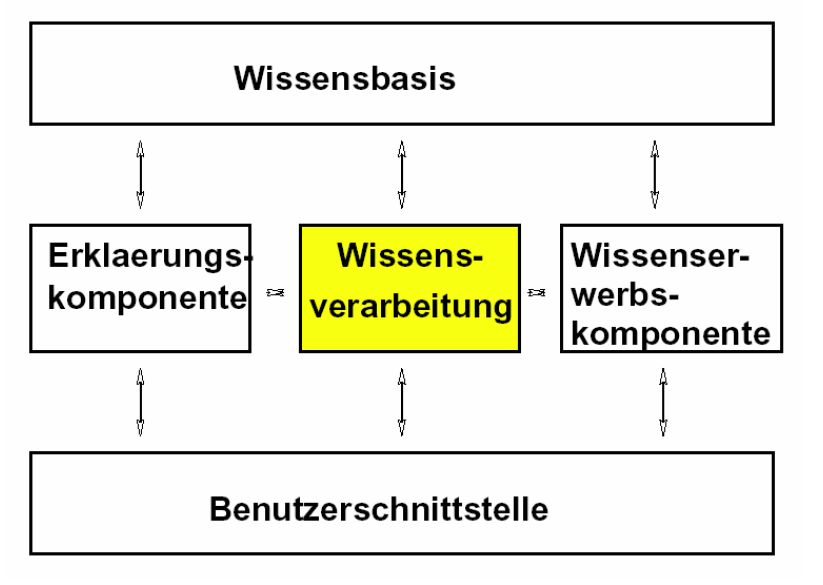
\includegraphics[width=250px]{images/expertensysteme}
\caption{Aufbau eines Expertensystems \cite[s.6]{bib:keller}}
\label{expert_system_structure}
\end{figure}

Die zentrale Komponente ist die \textit{Wissensverarbeitung}. Diese hat auf alle weiteren Komponenten Zugriff und interagiert mit diesen. Es werden die erhaltenen Fakten mithilfe der vorhandenen Regeln verknüpft. Aus der Verknüpfung werden neue Fakten gewonnen, die auf der \textit{Benutzerschnittstelle} angezeigt werden. Die Wissensbasis ist für das Speichern des Expertenwissens in Fakten und Regeln zuständig. Die Speicherung der Daten kann auf folgende zwei Arten geschehen\cite{bib:expert1}:\par
\begin{itemize}
        \item \textbf{generisch}: unabhängig vom aktuellen Anwendungsfall. Meist in einfachen Wenn-Dann-Regeln oder auf einem Modell beruhend. 
        \item \textbf{fallspezifisch}: zur Lösung eines konkreten Anwendungsfall
\end{itemize}
 Die Pflege dieser Basis erfolgt durch die \textit{Wissenserwerbskomponente}. Mit deren Hilfe lässt sich das vorhandene Expertenwissen in das System einpflegen. Die \textit{Erklärungskomponente} unterstützt das Nachvollziehen des Ergebnisses durch Erläuterungen zu den getätigten Entscheidungen.

\subsection{CAS Configurator Merlin Enterprise} \label{configurator}
Das Produkt CAS Configurator Merlin Enterprise ist die Konfigurationslösung der CAS Software AG für große Unternehmen. Das Produkt besteht aus einigen Standardkomponenten, die auf die einzelnen Bedürfnisse der Großkunden angepasst werden. In Abbildung \ref{airbus_structure} ist der Aufbau und das Zusammenspiel der verschiedenen Komponenten des Konfigurators zu sehen. \par
\begin{figure}
\centering
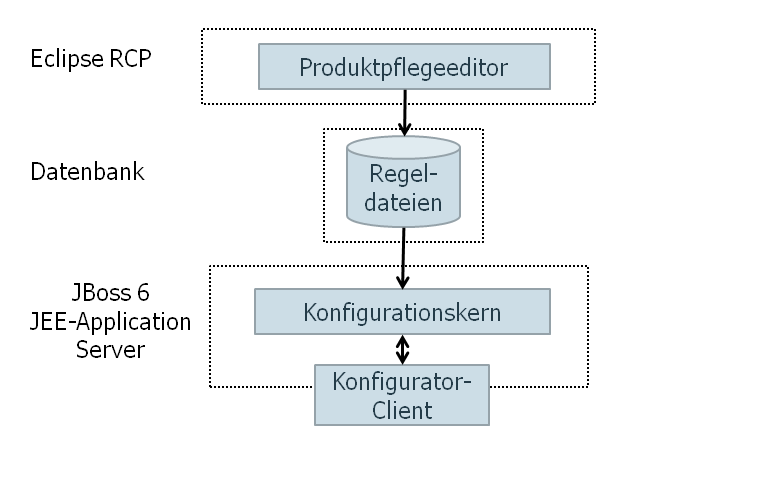
\includegraphics[width=\hsize]{images/AirbusAufbau}
\caption{Architektur der Airbus Komponenten}
\label{airbus_structure}
\end{figure}
Die Wissensverarbeitungs-Komponente aus Abschnitt \ref{konfiguratoren} ist hier der sogenannte \textit{Konfigurationskern}. Er ist für die Auswertung der getätigten Auswahl von Elementen des Produktes zuständig. Mithilfe von booleschen Regeln, welche mit dem \textit{Produktpflegeeditor} modelliert wurden und in einer \textit{Datenbank} gespeichert sind, wird die Auswahl verifiziert.
\par
 Der Konfigurationskern berechnet ebenfalls sogenannte Alternativen. Diese treten auf, sobald die derzeitige Selektion alleine, ohne Hinzunahme von weiteren Bauteilen, nicht umsetzbar ist. Der Konfigurator kann in diesem Fall neue Möglichkeiten (Alternativen) vorschlagen, damit die Konfiguration durchgeführt werden kann. Die Auswahl der Konfigurationselemente erfolgt im sogenannten Konfigurator-Client. Der Client ist mit der Benutzerschnittstelle im Expertensystem zu vergleichen. \par

Der Konfigurationskern, sowie der Client befinden sich auf einem Java-Applikations-Server. Der Produktpflegeeditor ist eine eigenständige Rich-Client Anwendung, welche auf dem Eclipse Rich-Client-Plattform Framework\cite{bib:eclipseRCP} basiert.

\subsection{Konfigurator des Kunden Airbus} \label{airbusConfigurator}
Die Arbeit wird speziell für den Flugzeughersteller Airbus\footnote{http://www.airbus.com/} angefertigt und beruht damit auf deren Konfigurationsmöglichkeiten. Airbus verwendet den Konfigurator für das Upgraden von bereits vorhandenen Flugzeugen einzelner Fluggesellschaften. Ein Beispiel für ein solches Upgrade können diverse Systemupgrades, wie bspw. ein neues Navigationssystem oder Ähnliches sein. Eine weitere Besonderheit im Konfigurationsrozess ist das Prüfen mit einzelnen Flugzeugen. Jedes verkaufte Flugzeug ist in der Datenbasis erfasst, sowie deren genaue Spezifikation und Bauteile. Der Konfigurator kann die Baubarkeit der einzelnen Upgrades genau auf ein bestimmtes Flugzeug prüfen lassen. \par

%TODO Beschreibung
 Bei der Modellierung von Konfigurationen werden sogenannte Status verwendet. Diese Status (engl. states) werden für Flugzeuge angelegt. Jeder einzelne Status repräsentiert eine erreichbare Konfiguration. Um einen Übergang zu einem state zu erreichen, wird ein bestimmtes Upgrade eingebaut  
 \par

Für die Konfiguration wird z.Zt. eine Weboberfläche als Konfigurations-Client verwendet. Diese Oberfläche ist sehr einfach gehalten und kann nur von Experten bedient werden, da mit einzelnen Produktcodes bei der Konfiguration gearbeitet wird. Die Weboberfläche befindet sich auf dem gleichen Applikationsserver wie der Kern und es besteht eine direkte Anbindung. In der Datenbank werden nicht nur Produkt- und Regelinformationen gehalten, sondern auch die Flugzeugdaten. 

  
\section{Grundlegende Anforderungen}
Die Anwendung ist kein vom Kunden vorgegebenes Projekt. Dies hat zur Folge, dass es keine strikten Anforderungen an die App gibt. Die Anwendung soll, wie in Abschnitt \ref{goal} festgelegt den Konfigurationsprozess des Kunden vereinfachen und "mobil" verfügbar machen. Der Prototyp soll den Kunden überzeugen, seinen derzeitigen Konfigurationsprozess in den Neuen zu überführen. Die Anforderungen an die Software müssen demnach so festgelegt werden, dass sie für eine hohe Akzeptanz beim Kunden sorgt. Damit die Anwendung akzeptiert wird, müssen alle Gütekriterien dieses Ziel verfolgen. \par

Die Festlegung der Kriterien ist nach Rücksprache mit den Entwicklern und dem Projektleiter des Kunden entstanden. Gemeinsam wurde eine Priorisierung der einzelnen Anforderungen entsprechend der Zielsetzung erarbeitet. Im Folgenden ist das Ergebnis in Funktionale und Nicht-Funktionale Anforderungen eingeordnet. Fachliche Funktionen der Anwendung sind in den funktionalen Anforderungen enthalten. Diese wurden anhand der bestehenden Software und den Möglichkeiten des Konfigurators erstellt. Weiterhin wurden zusätzlichen Anforderungen, aufgrund der mobilen Umgebung hinzugefügt . Bei den Nicht-Funktionalen Kriterien steht die Usability, das Anpassen auf die Umgebung , sowie die Kundenbegeisterung im Vordergrund. 

\subsection{Abgrenzung der Anforderungen}
Aufgrund der begrenzten Zeit im Rahmen dieser Arbeit wird die Anwendung prototypisch implementiert. Dies bedeutet, dass die Daten nicht vollständig sein müssen. Allerdings müssen die Daten in sich konsistent und auch an die Datenstruktur des Kunden angelehnt sein. Der Prototyp soll die Möglichkeiten einer mobilen Konfigurationslösung, auf den Kunden zugeschnitten zeigen. Für das Erreichen dieses Zieles werden zwei abgeschlossene Use-Cases bei innerhalb der Arbeit implementiert, die alle Funktionen der Anwendung beinhalten. Die Auswahl dieser Use-Cases ist Teil dieser Arbeit und wird im nächsten Kapitel beschrieben. \par

 Die bestehenden Funktionen des Konfigurationsservers werden verwendet. Es sind evtl. Anpassungen an die Reihenfolge der Aufrufe aufgrund der mobilen Zielumgebung notwendig. Um die Konfigurationsergebnisse empfangen zu können, soll eine einfache Webservicekommunikation mit dem Server stattfinden, die Kommunikationssicherung, wie Authentifizierung und Verschlüsselung ist nicht Teil der Arbeit. Dies soll bei einer späteren, vollständigen Implementierung berücksichtigt werden.

\subsection{Nicht-Funktionale Anforderungen}\label{non_functional_requirements}
\begin{tabular}[H]{| p{0.5cm} | p{2.2cm} | p{4.5cm} | p{5.3cm} | p{1.3cm} |}
\toprule[2pt] \rowcolor{dunkelgrau}
\hline
  NR. & Anforderung & Beschreibung & Details & Priorität \\
  \hline
  N1 & Einfache \newline Bedienung & Die Anwendung soll von unerfahrenen Benutzern schnell bedient werden können.& Schwerpunkte der Softwareergonomie\cite{bib:softwareErgonomie}: 
  \begin{itemize}
        \item Selbstbeschreibungs-fähigkeit
        \item Lernförderlichkeit
        \item Erwartungs-konformität
     \end{itemize}
   & A \\
  \hline
  N2 & Schnelle Bedienung & Die Auswahl der einzelnen Komponenten soll möglichst schnell getätigt werden können. & Es muss für eine flüssige Navigation zwischen den einzelnen Seiten gesorgt werden. Der Benutzer sollte keine langen Wartezeiten beim Bedienen der Anwendung haben. & A \\
  \hline
    N3 & Offline-Online Modus & Die Anwendung soll einen Offline- und Online-Modus enthalten & Es sollen Konfigurationsdaten offline zusammengestellt werden können, die später oder zeitgleich online (mit Konfigurationsserver) geprüft werden. & A \\
    \hline
    N4 & Allein-stellungs-merkmal & Um den Kunden zu begeistern ist ein besonderes Feature, welches die Anwendung als Alleinstellungsmerkmal besitzt wünschenswert.& Es sollen besonders "'aufregende"' Features, die eine Technologie bietet in die Anwendung integriert und in einem sinnvollen Kontext genutzt werden.  & B\\
    \hline
\bottomrule[2pt]
\end{tabular}

\subsection{Funktionale Anforderungen}
\begin{tabular}[H]{| p{0.4cm} | p{2.3cm} | p{4.5cm} | p{5.3cm} | p{1.3cm} |}
\toprule[2pt] \rowcolor{dunkelgrau}
\hline
  NR. & Anforderung & Beschreibung & Details & Priorität \\
  \hline
  F1 & Upgrade-auswahl & Es sollen Upgrades für Flugzeuge auswählbar sein & Bevor die Auswahl stattfindet, soll es verschiedene Filtermöglichkeiten geben, wie der Flugzeugtyp oder die Art des Upgrades.
   & A \\
  \hline
  F2 & Flugzeug-auswahl & Es müssen Flugzeuge eines bestimmten Kunden auswählbar sein. & Es soll auch hier, analog zu B1 die Möglichkeit der Auswahl von Flugzeugen auf einen vorher gefilterten Datensatz geben. & A \\
  \hline
    F3 & Konfiguration & Nach erfolgter Auswahl werden die Ergebnisse der Konfiguration dargestellt. & Kommunikation mit dem Konfigurationsserver, sowie die Darstellung der Ergebnisse auf dem Client& A \\
    \hline
     F4 & Alternativen & Bei mehreren Möglichkeiten einer Auswahl sollen Alternativen ausgewählt werden können & Übersichtliche Darstellung von Alternativenauswahl.& A \\
        \hline
    F5 & Speichern & Die getätigte Auswahl soll gespeichert werden& Nach Abschluss der Konfiguration soll diese lokal gespeichert werden, um ein erneutes Laden zu ermöglichen. & B\\
    \hline
    F6 & Laden & Getätigte Konfigurationen müssen geladen werden können& Beim Start der Anwendung sollen getätigte Konfigurationen geladen und angezeigt werden können & B\\
    \hline
\bottomrule[2pt]
\end{tabular}





